% !TeX spellcheck = en_US	

\documentclass[10pt,journal,compsoc]{IEEEtran}
\usepackage{graphicx}
\usepackage[ruled, linesnumbered]{algorithm2e}
\usepackage{url}
\usepackage{epstopdf}
\usepackage{indentfirst}
\usepackage[tight,footnotesize]{subfigure}
\usepackage{amsmath}
\usepackage{amssymb}
\usepackage{multirow}
\usepackage{color}
\usepackage{enumerate}

\newtheorem{theorem}{Theorem}[section]
\newtheorem{lemma}[theorem]{Lemma}
\newtheorem{observation}[theorem]{Observation}
\newtheorem{corollary}[theorem]{Corollary}

% *** CITATION PACKAGES ***
\ifCLASSOPTIONcompsoc
\usepackage[nocompress]{cite}
\else
\usepackage{cite}
\fi

\begin{document}

\title{Building and Checking Suffix Array Using Induced Sorting Method}

\author{Yi~Wu,
	Ge~Nong,
	Wai~Hong~Chan,
	and~Bin~Lao
	\IEEEcompsocitemizethanks{
		\IEEEcompsocthanksitem Y. Wu, G. Nong (corresponding author) and B. Lao are with the Department of Computer Science, Sun Yat-sen University, Guangzhou 510275, China. E-mails: wu.yi.christian@gmail.com, issng@mail.sysu.edu.cn, Laobin@mail3.sysu.edu.cn.
		
		\IEEEcompsocthanksitem Wai Hong Chan (corresponding author) is with the Department of Mathematics and Information Technology, The Education University of Hong Kong, Hong Kong. E-mail: waihchan@ied.edu.hk.
}}% <-this % stops a space


\IEEEtitleabstractindextext{% 
\begin{abstract}

In the past decade, the induced sorting~(IS) method has been successively used to design disk-based suffix array~(SA) construction algorithms that have better time and I/O complexities than the existing alternatives. However, their current programs commonly suffer from a performance bottleneck due to large disk space in need. Recently, it was reported a carefully engineered IS suffix sorter that takes less than $8n$ disk space for constructing an SA encoded by 40-bit integers. This indicates a great potential for improving space efficiency of the prior arts, such as DSA-IS and SAIS-PQ. In this paper, we present a checking method that enables any IS suffix sorting algorithms to check an SA when it is being built. For performance analysis, we integrate the proposed method into DSA-IS and implement the enhanced algorithm to evaluate the checking overhead, where the program design of DSA-IS has been optimized for a better speed and smaller peak disk use. From our experiments, the time, space and I/O consumptions for verification is negligible in comparison with that for construction. In view of the high performance of this checker and the existing IS suffix sorters, we are convinced that our checking method, in accompanied with the state-of-the-art IS suffix sorting algorithm, can constitute an efficient solution to the situations where checking is a must for a constructed SA.

\end{abstract}

% Note that keywords are not normally used for peerreview papers.
\begin{IEEEkeywords}
Suffix array, construction and verification, external memory.
\end{IEEEkeywords}}


% make the title area
\maketitle

\IEEEdisplaynontitleabstractindextext

\IEEEpeerreviewmaketitle

\section{Introduction}\label{sec:introduction}

Given a string drawn from a constant or integer alphabet, its suffix array can be built by the internal-memory algorithm SA-IS~\cite{Nong11} in linear time and space. So far, the IS method has been also applied to designing three external-memory suffix sorting algorithms~eSAIS~\cite{Bingmann12}, DSA-IS~\cite{Nong15} and SAIS-PQ~\cite{Liu15}, which have better time and I/O complexities than other alternatives, e.g., DC3~\cite{Dementiev2008a}, bwt-disk~\cite{Ferragina2012}, SAscan~\cite{Karkkainen2014} and pSAscan~\cite{Karkkainen2015}. However, the peak disk uses of their current programs are at least 15 times the sizes of input strings, resulting in a performance bottleneck. Recently, it was reported in~\cite{Karkkainen2017} a new IS suffix sorting algorithm fSAIS with a careful engineering that consumes nearly optimal disk space and runs faster than the parallel suffix sorter pSAscan on massive datasets. The algorithmic design of fSAIS is highly dependent on that of the prior arts. Particularly, it employs a sorting method similar to that of DSA-IS for inducing suffixes/substrings and the naming method of SAIS-PQ for producing reduced strings. The substantial improvement on space efficiency is mainly achieved by means of a monotone priority queue  for sorting substrings/suffixes and a garbage collector for quickly recycling disk space occupied by data no longer to use. As a result, its implementation takes less than $8n$ disk space for any input string of a size $n \le 2^{40}$, indicating a great potential for optimizing the programs for DSA-IS and SAIS-PQ. In this paper, we make our first attempt to redesign DSA-IS using new substring sorting and naming methods. The experimental results indicate that our program for the enhanced algorithm consumes about two-thirds as much disk space as that for eSAIS and runs faster than the latter on real world datasets. In addition, we also give a discussion on further improving our program to achieve a better space efficiency using the techniques for implementing fSAIS.

To detect potential computation errors caused by implementation bugs and/or hardware malfunctions, a constructed SA should be verified to ensure its correctness before use. This checking function has been included into various widespread software packages like SA-IS, DC3 and eSAIS. Particularly, the latter two verify an SA using the checking method presented in~\cite{Dementiev2008a}, which mainly consists of two passes of external-memory sorts involving $\mathcal{O}(n)$ fixed-size tuples with an integer key. In this paper, we propose a new checking method that enables any IS suffix sorting algorithm to check an SA when it is being built. 
For performance analysis, we integrate the proposed method into the optimized DSA-IS and implement the combined algorithm, called DSA-IS+, to evaluate the checking overhead. From our experiments, the time, space and I/O consumptions for verification is negligible in comparison with that for construction. In view of the high performance of this checker and the existing IS suffix sorters, we believe that our checking method, together with the state-of-the-art IS suffix sorting algorithm, can constitute an efficient solution to the situations where checking is a must for a constructed SA.

The rest of the paper is organized as follows. We first describe in Sections~\ref{sec:build_sa} and~\ref{sec:check_sa} the adapted algorithmic design of DSA-IS and the proposed checking method, respectively. Then, we demonstrate the experimental results in Section~\ref{sec:experiments} and draw the concluding remarks in Section~\ref{sec:conclusion}.


\section{SA Builder}~\label{sec:build_sa}

\subsection{Preliminaries}

Given an input string $x[0, n)$ with a unique smallest character $x[n - 1]$, we denote by ${\sf suf}(i)$ a suffix starting with $x[i]$ and ${\sf sub}(i,j)$ a substring running from $x[i]$ to $x[j]$. The following notations are used in our presentation for denotation convenience.

Character/substring/suffix classification. Characters of $x$ are classified into two categories: L-type and S-type. To be specific, $x[i]$ is S-type if (1) $i = n - 1$ or (2) $x[i] = x[i + 1]$ and $x[i + 1]$ is S-type; otherwise, $x[i]$ is L-type. Particularly, if $x[i]$ and $x[i - 1]$ are respectively S-type and L-type, then $x[i]$ is also S*-type. In addition, a substring/suffix is of the same type as its heading character. We use an integer array $t$ to indicate the type of characters, where $t[i] = 1$ or $0$ if $x[i] $ S-type or L-type, respectively.

Predecessor and Successor. For any two neighboring characters $x[i]$ and $x[i + 1]$, we say $x[i]$ is the predecessor of $x[i + 1]$ while the latter is the successor of the former. Similarly, there also exists a predecessor-successor relationship between ${\sf suf}(i)/{\sf sub}(i, j)$ and ${\sf suf}(i + 1)/{\sf sub}(i + 1, j)$.

\subsection{Overview of DSA-IS} \label{subsec:improvement}



% Algorithm
\begin{algorithm*}
	\SetAlgoNoLine
	\KwIn{$x$}
	\KwOut{$x_1$}
	
	$r := 0$ \label{alg1:1}
	
	\For{$i := n - 1; i \ge 0; i := i - 1$}{
		
		\If{$t[i] = 1$ and $t[i - 1] = 0$}{ 
			
			$PQ_1.{\sf push}(\langle x[i], t[i], r, i\rangle)$ // sort S*-type characters 
		}
	}\label{alg1:2}
	
	\While{$PQ_1.{\sf notEmpty}()$}{ \label{alg1:3}
		
		$top = PQ_1.{\sf top}(), PQ_1.{\sf pop()}, r:= r + 1$
		
		$pos = top.4th, ch = top.1st, pre\_ch = {\sf getPrecCh}(pos)$  // retrieve the heading character of the predecessor
		
		\If{$top.2nd = 0$ and $pre\_ch \ge ch$ or $top.2nd = 1$ and $pre\_ch > ch$}{
			
			$PQ_1.{\sf push}(\langle pre\_ch, 1, r, pos  - 1 \rangle)$ // induce the L-type predecessor
		}
		\Else{
			$PQ_2.{\sf push}(\langle ch, 1, r, pos \rangle)$ // keep the sorted L*-type substrings
		}
	} \label{alg1:4}
	
	$r := n$  \label{alg1:5}
	\While {$PQ_2.{\sf notEmpty}()$}{
		
		$top = PQ_2.{\sf top}(), PQ_2.{\sf pop()}, r := r - 1$
		
		$pos = top.4th, ch = top.1st, pre\_ch = {\sf getPrecCh}(pos)$  // retrieve the heading character of the predecessor
		
		\If{$top.2nd = 1$ and $pre\_ch \le ch$ or $top.2nd = 0$ and $pre\_ch < ch$}{
			
			$PQ_2.{\sf push}(\langle pre\_ch, 1, r, pos  - 1\rangle)$ // induce the S-type predecessor
		}
		\Else{
			
			$Vec.{\sf push\_back}(pos)$ // keep the sorted S*-type substrings
		}
	} \label{alg1:6}
	
	
	$last\_str := 0, last\_pos = n - 1, name = 0$ \label{alg1:7}
	
	\While {$Vec.{\sf notEmpty}()$}{ 
		
		$pos = Vec.{\sf pop\_back}(), str := {\sf getStr}(pos)$ // get S*-type substring
		
		\If{$last\_str \ne str$}{
			
			$name := name + 1$ // literally compare two lexicographically neighboring substrings 
		}
		
		$Sorter.{\sf push}(\langle pos, name\rangle)$
		
		$last\_pos = pos, last\_str = str$
	} \label{alg1:8}
	
	$Sorter.sort()$  \label{alg1:9}
	
	\For{$i := 0; Sorter.{\sf notEmpty}(); i:= i + 1$}{
		
		$x_1[i] = Sorter.2nd, Sorter.{\sf next}()$ // produce the reduced string
		
	} \label{alg1:10}
	
	
	\caption{The Reduction Phase for an IS Suffix Sorting Algorithm.}
	
	\label{alg:1}
\end{algorithm*}

An IS suffix sorting algorithm mainly consists of a reduction phase for sorting S*-type substrings and an induction phase for sorting suffixes. Both two phases execute the same process to accomplish the sorting tasks, while the reduction phase additionally performs a naming process to produce a reduced string $x_1$. For a better understanding, we illustrate in Algorithm~\ref{alg:1} the details of the reduction phase and summarize the framework below, where $PQ_1$ and $PQ_2$ are two priority queues with a sorting key consisting of the first three components. 

\begin{enumerate}[S1]

\item Scan $x$ to find S*-type characters and insert them into $PQ_1$. (lines~\ref{alg1:1}-\ref{alg1:2}) \label{reduction_phase_framework:1}

\item Sequentially access the sorted substrings popped from $PQ_1$ in ascending order to induce their L-type predecessors, where each induced L-type substring is pushed into $PQ_1$ and each scanned L*-type substring is pushed into $PQ_2$ for later use. (lines~\ref{alg1:3}-\ref{alg1:4}) \label{reduction_phase_framework:2}

\item Sequentially access the sorted substrings popped from $PQ_2$ in descending order to induce their S-type predecessors, where each induced S-type substring is pushed into $PQ_2$ and each scanned S*-type substring is appended to a vector $Vec$. (lines~\ref{alg1:5}-\ref{alg1:6}) \label{reduction_phase_framework:3}

\item Compare the sorted S*-type substrings in $Vec$ to assign them names, where the name for each substring indicates it relative order among all. (lines~\ref{alg1:7}-\ref{alg1:8}) \label{reduction_phase_framework:4}

\item Sort the names in position order to produce the reduced string $x_1$. (lines~\ref{alg1:9}-\ref{alg1:10}) \label{reduction_phase_framework:5}

\end{enumerate}

It should be noticed that S\ref{reduction_phase_framework:2} and S\ref{reduction_phase_framework:3} induce the order of unsorted substrings from that of their heading characters and successors. When finished these two steps, all the S*-type substrings are sorted in their lexical order and stored in $Vec$. S\ref{reduction_phase_framework:4} performs a naming process to literally compare each pair of neighbors in the vector and assign them the same or different names with respect to whether they are equal or not. After that, S\ref{reduction_phase_framework:5} replaces each S*-type substring with its name to produce the reduced string $x_1$. 

Algorithm~\ref{alg:1} can be implemented in external memory by sequential I/O operations except when calling ${\sf getPrecCh}$ or ${\sf getStr}$. These two functions invoke a random disk access per execution and thus may lead to a performance bottleneck. The existing disk-based IS suffix sorting algorithms adopt different approaches to amortize the I/O overhead. For DSA-IS, it employs an internal-memory preprocessor to prefetch the required data and sort them in their access order before use. In general, it first divides the input string into $\mathcal{O}(n/M)$ blocks consisting of one or multiple successive S*-type substrings. Then, it loads each block into RAM and sorts the S*-type substrings in the block following the same idea of S\ref{reduction_phase_framework:2}-S\ref{reduction_phase_framework:5}, where it records the returns of ${\sf getPrecCh}$ and ${\sf getStr}$ during the sort. Afterward, it executes Algorithm~\ref{alg:1} to sort all the S*-type substrings and retrieves the preceding characters and the target substrings from the block-wise results by sequential I/O operations.

\subsection{Improvements on Design of DSA-IS}

Recall that Algorithm~\ref{alg:1} performs the sorting and naming processes in sequence. Our first improvement is to reuse the substring naming method originally proposed for SAIS-PQ to combine the execution of these two processes during the reduction phase. In Algorithm~\ref{alg:1}, two priority queues are employed to sort substrings according to their heading characters and the rank of their successors, where the rank value indicates the access order of the corresponding substring. Notice that the lexical order of any two substrings/suffixes can be determined by that of their heading characters and successors as well, thus the priority queues can sort substrings by their names instead of their ranks. The name of currently scanned L-type/S-type substring can be computed by comparing its heading character and the name of its successor with that of the last scanned L-type/S-type substring. If both are equal, then the two substrings have the same name; otherwise, the former is assigned a name bigger/smaller than the latter. 

From our experiments, sorting substrings by the priority queues takes long CPU time and large I/O volume. To reduce the consumption, we present a new method that combines the sorted S*-type substrings of all the blocks by a merger, which maintains a buffer for each block to preload the sorted S*-type substrings into RAM and an internal-memory heap to compare the substrings belonging to different blocks by literal comparisons. For the substrings too long to be wholly loaded into RAM, this method first uses the priority queue to sort them in external memory and then employs the merger to compare them with the short substrings based on the following property: suppose $sub_a$ and $sub_b$ are respectively long and short substrings, then $sub_a < sub_b$ if (1) $sub_a[0, D) = sub_b$ or (2) $sub_a[0, k) = sub_b[0, k)$ and $sub_af_a[k] < sub_b[k]$, where $D = \|sub_b\|$ and $k < D$. This indicates that we only need to fetch the first $D$ characters of a long substring into RAM when comparing it with a short substring containing $D$ characters. 

\subsection{Discussion} \label{subsec:further_discussion}

As demonstrated in Section~\ref{sec:experiments}, our implementation for the enhanced DSA-IS has an advantage over that for eSAIS in terms of time, space and I/O volume, but its peak disk use remains at a high level. This is mainly because it fails to gradually clean up the temporary data when they are being used. On the contrary, fSAIS stores the temporary data using multiple files and deletes each file immediately when all that residing on it is longer to use. Therefore, it is reasonable to believe that our program can achieve a substantial improvement following the same technique. Currently, we are attempting to further improve the algorithmic and implementation designs of DSA-IS. 

\section{SA Checker}~\label{sec:check_sa}

\subsection{Details} 

A constructed SA should be verified to ensure its correctness before use. This checking function can be found in some widespread software packages like SA-IS, DC3 and eSAIS, where the latter two perform verification based on Theorem~\ref{theorem:1}.

\begin{theorem} \label{theorem:1}
	$sa[0, n)$ is the SA for $x[0, n)$ if and only if the following conditions are satisfied:\\
	(1) $sa$ is a permutation of $[0, n)$. \\	
	(2) ${\sf r_i < r_j} \Leftrightarrow (x[i], r_{i + 1}) < (x[i], r_{j + 1})$ for $ i, j \in [0, n)$ and $i\ne j$, where $r_i$ and $r_j$ indicates the relative order of ${\sf suf}(i)$ and ${\sf suf}(j)$ among all the suffixes, respectively. \\
\end{theorem}

\begin{IEEEproof}
	The proof is available in~\cite{Dementiev2008a}.
\end{IEEEproof}

This method executes two passes of integer sorts and each sort involves $n$ fixed-size tuples, thus it takes large disk space and I/O volume when implemented in the external memory, resulting in a non-negligible checking overhead. Take eSAIS for example, the peak disk use for sequentially building and checking SA rises up to $27n$, while the I/O volume also increases by $50n$. 


We propose a fast and lightweight SA checking method that can be seamlessly integrated into any IS suffix sorting algorithms for building and checking an SA simultaneously. Before presentation, we introduce two lemmas that will be used to prove the correctness of our checking method. Both two Lemmas demonstrate the fact that the lexical order of two suffixes can be determined by their heading characters and successors. Particularly, Lemma~\ref{lemma:2} is applied to any IS suffix sorting algorithm for inducing unsorted suffixes from sorted ones during the induction phase.

\begin{lemma} \label{lemma:1}
	For $i, j \in [0, n)$ and $i \ne j$, ${\sf suf}(i) < {\sf suf}(j) \Leftrightarrow (x[i], {\sf suf}(i + 1)) < (x[j], {\sf suf}(j + 1))$.
\end{lemma}

\begin{lemma} \label{lemma:2}
	For $i, j \in [0, n)$ and $i \ne j$, $r_i < r_j \Leftrightarrow (x[i], r_{i + 1}) < (x[j], r_{j + 1})$, where $r_i$ and $r_j$ indicates the relative order of ${\sf suf}(i)$ and ${\sf suf}(j)$ among all the suffixes, respectively.
\end{lemma}

In what follows, we use the above lemmas to prove Theorem~\ref{theorem:2}, where $sa^*_1$ and $sa^*_2$ are two integer arrays that record the starting positions of the sorted S*-type suffixes. To be specific, the former is computed from the SA for $x_1$ and the latter is retrieved from the final SA for $x$. 

\begin{theorem} \label{theorem:2}
	For any IS suffix sorting algorithm, its output $sa[0, n)$ is the SA for the input string $x[0,n)$ if and only if the following conditions are satisfied: \\
	(1) $sa^*_1[i] \ne sa^*_1[j]$ for $i, j \in [0, n)$ and $i \ne j$. \\
	(2) $sa^*_1 = sa^*_2$. \\
\end{theorem}

\begin{IEEEproof}
	We only prove the sufficiency as the necessity is clear.
	
	Suppose $sa$ is not a permutation of $[0, n)$. Without loss of generality, let $i \ne j$ and $sa[i] = sa[j]$, then $u \ne v$ and $sa[u] = sa[v]$ according Lemma~\ref{lemma:2}, where ${\sf suf}(sa[u])$ and ${\sf suf}(sa[v])$ are the successors of ${\sf suf}(sa[i])$ and ${\sf suf}(sa[j])$, respectively. By recursively replacing $(i, j)$ with $(u, v)$, we can find two elements $sa[i_0]$ and $sa[j_0]$ storing the starting position of the same S*-type suffix. This indicates that $sa^*_1$ contains duplicate elements, which violates condition (1) in Theorem~\ref{theorem:2}.
	
	Suppose $i < j$ and ${\sf suf}(sa[i]) > {\sf suf}(sa[j])$. If $x[sa[i]] < x[sa[j]]$, then ${\sf suf}(sa[i]) < {\sf suf}(sa[j])$ according to Lemma~\ref{lemma:1}; otherwise, if $x[sa[i]] > x[sa[j]]$, then $i > j$ according to Lemma~\ref{lemma:2}. Both lead to a contradiction. Given that $x[sa[i]] = x[sa[j]]$, then $u < v$ and ${\sf suf}(u) > {\sf suf}(v)$, where ${\sf suf}(sa[u])$ and ${\sf suf}(sa[v])$ are the successors of ${\sf suf}(sa[i])$ and ${\sf suf}(sa[j])$, respectively. By recursively replacing $(i, j)$ with $(u, v)$, we can find two elements $sa[i_0]$ and $sa[j_0]$ such that at least one stores the starting position of an S*-type suffix. We continue the proof following one of the three cases below:
	\begin{enumerate}[(1)]
	\item $x[sa[i_0]]$ is S*-type and $x[sa[j_0]]$ is L-type. In this case, $x[sa[i_0] + 1] > x[sa[j_0] + 1]$. Therefore, $u_0 > v_0$ according to Lemma~\ref{lemma:2}. This indicates that $(x[sa[i_0]], u_0) > (x[sa[j_0]], v_0)$ and thus $i_0 > j_0$ according to Lemma~\ref{lemma:2}. This leads to a contradiction.
	\item $x[sa[i_0]]$ is L-type and $x[sa[j_0]]$ is S*-type. In this case, $x[sa[i_0] + 1] < x[sa[j_0] + 1]$. Therefore, ${\sf suf}(sa[u_0]) < {\sf suf}(sa[v_0])$ according to Lemma~\ref{lemma:1}. This indicates that $(x[sa[i_0]], {\sf suf}(sa[u_0])) < (x[sa[j_0]], {\sf suf}(sa[v_0])$ and thus ${\sf suf}(sa[i_0]) < {\sf suf}(sa[j_0])$ according to Lemma~\ref{lemma:1}. This leads to a contradiction.
	\item $x[sa[i_0]]$ and $x[sa[j_0]]$ are both S*-type. Let $(i_0, j_0)$ be the pair that maximize $sa[i_0] + sa[j_0]$ such that $i_0 < j_0$ and ${\sf suf}(sa[i_0]) > {\sf suf}(sa[j_0])$, then $u_0 > v_0$ and ${\sf suf}(sa[u_0]) > {\sf suf}(sa[v_0])$. \footnote{Notice that $(u_0, v_0)$ must exist because the sentinel is a size-one S*-type substring smaller than others.} Because $x[i_0, u_0) = x[j_0, v_0)$, there must be $i_0 > j_0$ according to Lemma~\ref{lemma:2}. This contradiction indicates that $sa^*_1$ and $sa^*_2$ differ from each other, which violates condition (2) in Theorem~\ref{theorem:2}.
	\end{enumerate}

\end{IEEEproof}


The first condition in Theorem~\ref{theorem:2} can be easily checked when computing $sa^*_1$ from $sa_1$. For the second condition, a naive method is to first make a copy of $sa^*_1$ and $sa^*_2$ when inducing $sa$ and then sequentially compare their elements after the induction phase. This method takes linear time, space and I/O overhead. A more efficient alternative is to compute and compare the fingerprints for these two arrays, denoted by ${\sf fp}(sa^*_1)$ and ${\sf fp}(sa^*_2)$, instead to determine their equality. Obviously, $sa^*_1$ and $sa^*_2$ share a common fingerprint if they are equal to each other, but the inverse is not always true. Fortunately, by using the fingerprinting function described in~\cite{Karp1987}, the probability of a false match can be reduced to a completely negligible level. The above discussion leads us to the following statement.

\begin{corollary} \label{theorem:3}
	For any IS suffix sorting algorithm, its output $sa[0, n)$ is the SA for the input string $x[0, n)$ with a high probability if the following conditions are satisfied:
	(1) $sa^*_1[i] \ne sa^*_1[j]$ for $i, j \in [0, n)$ and $i \ne j$. \\
	(2) ${\sf fp}(sa^*_1) = {\sf fp}(sa^*_2)$. \\
\end{corollary}


\subsection{Example} \label{sec:check_sa:example}

xxxx


\section{Experiments} \label{sec:experiments}

For performance evaluation, we engineer DSA-IS and its optimized DSA-IS+, by using the STXXL's containers~(sorter, priority queue, vector and stream) to conduct efficient I/O operations in the external memory. As reported in~\cite{Karkkainen2014}, SAscan outperforms eSAIS in practice when the internal memory capacity $M$ is adequate. However, the time and space complexities of the program for SAscan are $\widetilde{\mathcal{O}}(n^2/ M)$ and $\widetilde{\Omega}(n^2/ M)$, respectively, thus it will suffer from a performance degradation as the size of the input string gets larger.\footnote{The authors in~\cite{Karkkainen2015} says, "SAscan needs just 7.5n bytes of disk space but because of its $\widetilde{\mathcal{O}}(n^2/ M)$ time complexity, it is competitive with eSAIS only when the input is less than about five times the size of RAM.".} On the other hand, the programs for DSA-IS, DSA-IS+ and eSAIS\footnote{https://panthema.net/2012/1119-eSAIS-Inducing-Suffix-and-LCP-Arrays-in-External-Memory/} are not only of linear I/O volume and space complexities in theory, but also commonly implemented by the STXXL library. \textbf{Therefore, we use eSAIS rather than SAscan as a baseline for evaluating the performance of DSA-IS and DSA-IS+.} The experimental platform is a desktop computer equipped with an Intel Xeon E3-1220 V2 CPU, 4GiB RAM and 500GiB HD. The programs are complied by gcc/g++ 4.8.4 with -O3 options under Ubuntu 14.04 64-bit operating system.

In our experiments, three performance metrics are investigated for the programs running on the corpora listed in Table~\ref{tbl:corpora}, where each metric is measured as a mean of two runs of the programs.

\begin{itemize}
	\item construction time~(CT): the running time, in units of microseconds per character.
	\item peak disk usage~(PDU): the maximum disk space requirement, in units of bytes per character.
	\item I/O volume~(IOV): as the term suggests, in units of bytes per character.
\end{itemize}

%Table
\renewcommand\arraystretch{1.3}
\begin{table*}[!t]
	\caption{Corpus, $n$ in Gi, 1 byte per character} 
	\label{tbl:corpora}
	\centering
	\begin{tabular}{|l|c|c|p{10cm}|}
		\hline
		Corpora & \multicolumn{1}{c|}{$n$} & \multicolumn{1}{c|}{$\|\Sigma\|$} & Description \\\hline
		guten & 22.5 & 256 & Gutenberg, at \url{http://algo2.iti.kit.edu/bingmann/esais-corpus}.\\\hline 				
		enwiki & 74.7 & 256 & Enwiki, at \url{https://dumps.wikimedia.org/enwiki}, dated as 16/05/01. \\\hline	
		proteins & 1.1 & 27 & Swissprot database, at \url{http://pizzachili.dcc.uchile.cl/texts/protein}, dated as 06/12/15. \\\hline
		uniprot & 2.5 & 96 & UniProt Knowledgebase release 4.0, at \url{ftp://ftp.expasy.org/databases/.../complete}, dated as 16/05/11. \\\hline
		genome & 2.9 & 6 & Human genome data, used in Dementiev et al.~\cite{Dementiev2008a}, at \url{http://algo2.iti.kit.edu/dementiev/esuffix/instsances.shtml.} \\\hline
	\end{tabular}
\end{table*}

\subsection{Performance Evaluation on Construction Algorithms}
Figure~\ref{fig:performance_analysis1} illustrates the performance of the programs for DSA-IS and eSAIS in terms of the investigated three metrics, where guten\_14G and enwiki\_14G are prefixes of the corresponding corpus. As depicted, the peak disk usage for DSA-IS is around $16n$ on the two datasets, which is two-thirds of that for eSAIS. However, eSAIS outperforms DSA-IS with respect to the construction time, where the speed gap between them is mainly due to the different I/O volumes taken by the two algorithms. In order for a deep insight, we show in Table~\ref{tbl:volume_cmp} the statistics for I/O volumes of the algorithms in their reduction and induction phases. It can be observed that, although the I/O volumes spent in the induction phase are similar, eSAIS is far more I/O-efficient than DSA-IS when sorting substrings during the reduction phase. More specifically, the ratio of reduction and induction volumes for DSA-IS is about 0.80 while the counterpart for eSAIS is 0.23.

\begin{figure}[htbp!]
	\centering
	\subfigure{
		\label{subfig:pdu_cmp1}
		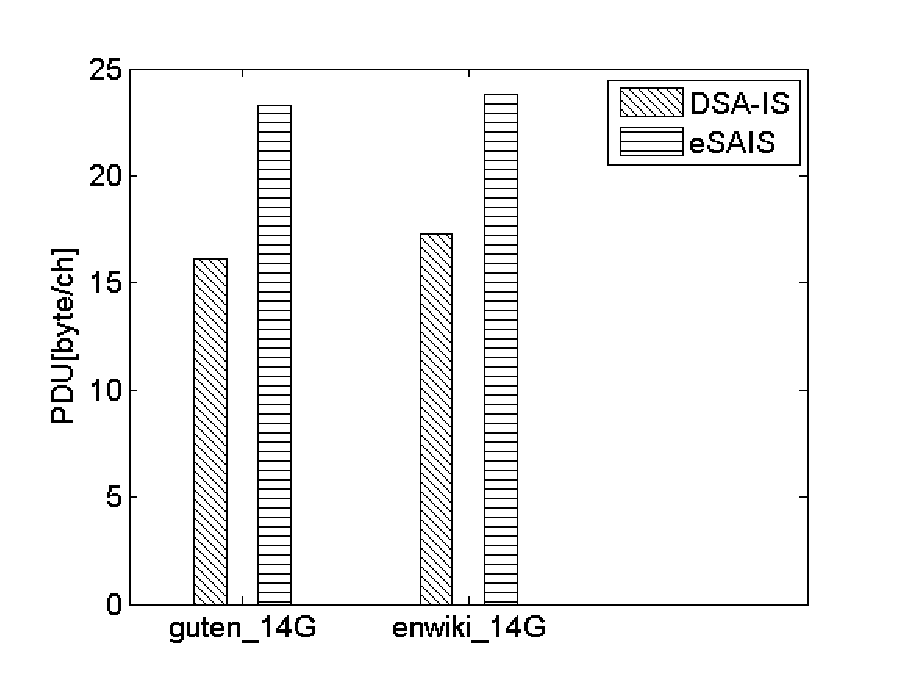
\includegraphics[width = 0.9\columnwidth]{pdu_cmp1}
	}
	\hfil
	\subfigure{
		\label{subfig:iov_cmp1}
		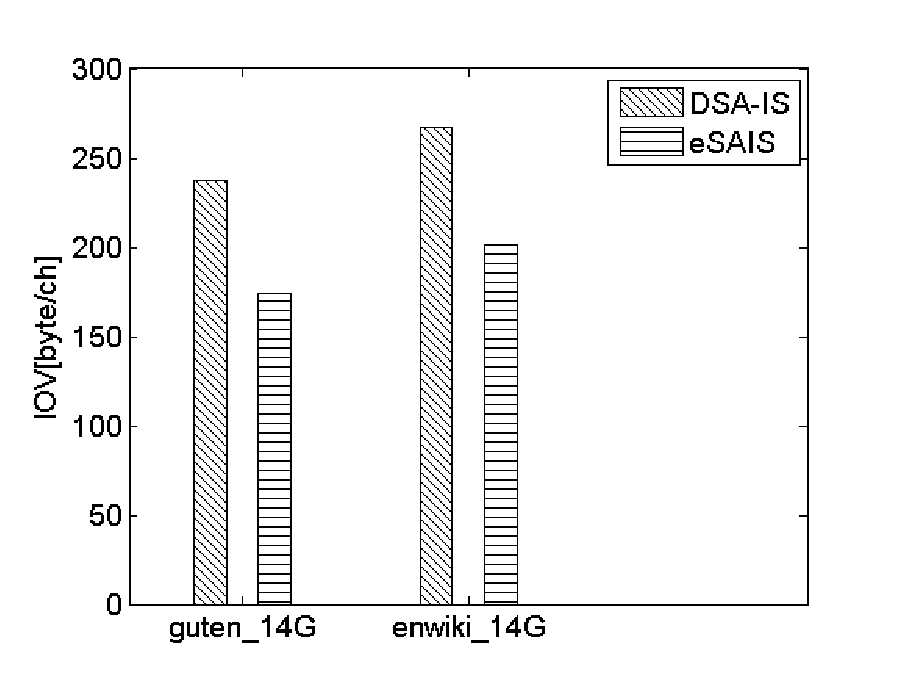
\includegraphics[width = 0.9\columnwidth]{iov_cmp1}
	}
	\hfil
	\subfigure{
		\label{subfig:ct_cmp1}
		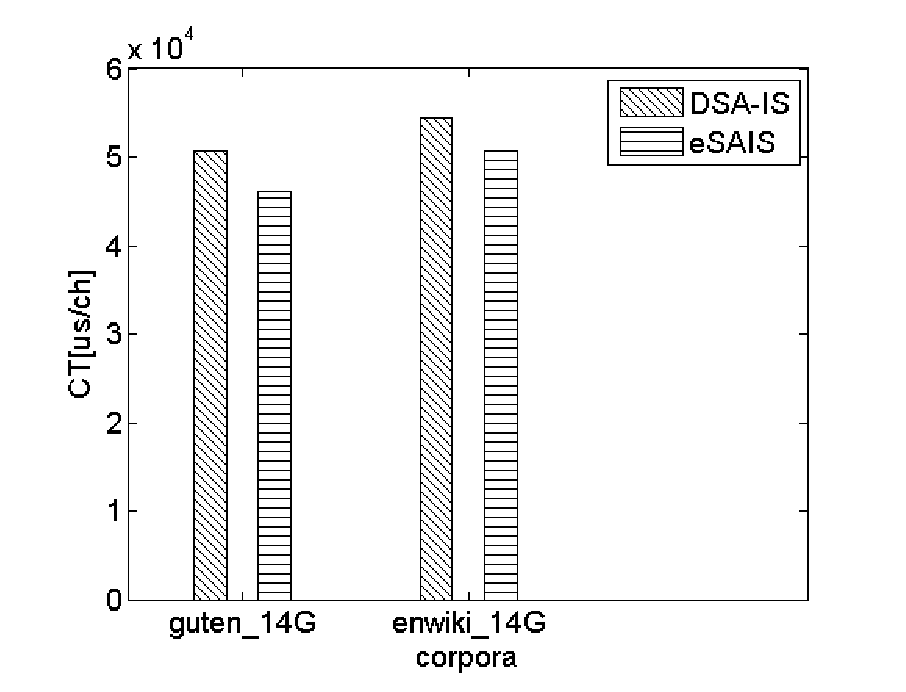
\includegraphics[width = 0.9\columnwidth]{ct_cmp1}
	}
	\caption{Experimental results for DSA-IS and eSAIS on guten\_14G and enwiki\_14G in terms of peak disk usage, I/O volume and construction time.}
	\label{fig:performance_analysis1}
\end{figure}

% Table
\begin{table*}%
	\caption{Comparison of Reduction and Induction I/O Volumes Amongst DSA-IS, DSA-IS+ and eSAIS on enwiki}
	\label{tbl:volume_cmp}
	\centering
	\begin{tabular}{|c|c|c|c|c|c|c|c|c|c|c|c|c|}
		\hline
		\multicolumn{1}{|c}{} & \multicolumn{4}{|c|}{eSAIS} & \multicolumn{4}{c|}{DSA-IS} & \multicolumn{4}{c|}{DSA-IS+ ($D_1 = 8$, $D_2 = 10$)}\\\hline
		\hline
		Size & Red. & Ind. & Total & Ratio & Red. & Ind. & Total & Ratio & Red. & Ind. & Total & Ratio\\\hline
		1G & 36.6 & 132.8 & 169.4 & 0.27 & 81.3 & 105.9 & 187.2 & 0.76 & 39.1 & 104.3 & 143.4 & 0.37\\\hline
		2G & 36.0 & 141.9 & 177.9 & 0.25 & 83.5 & 108.2 & 191.7 & 0.77 & 37.8 & 106.4 & 144.2 & 0.35\\\hline
		4G & 35.6 & 152.1 & 187.7 & 0.23 & 94.3 & 118.9 & 213.2 & 0.79 & 42.4 & 117.0 & 159.4 & 0.36\\\hline
		8G & 35.2 & 165.7 & 200.9 & 0.21 & 107.8 & 132.3 & 240.1 & 0.81 & 43.7 & 129.9 & 173.6 & 0.33\\\hline
		14G & 35.0 & 172.1 & 207.1 & 0.20 & 121.9 & 146.6 & 268.5 & 0.83 & 43.8 & 142.3 & 186.1 & 0.30\\\hline
	\end{tabular}
\end{table*}%

The above phenomenon can be explained as follows. During the reduction phase, DSA-IS partitions the input string $x$ into multiple blocks and induced sorts the substrings of each block in the internal memory. Then it reuses the induced sorting method to sort all the substrings of $x$ in the external memory by merging the block-wise results residing on disks. In contrast with DSA-IS, eSAIS splits $x$ into fixed-size partitions and sorts the substrings of each partition in the internal memory by calling std::sort. Then, it generates the global result by merging the partial ones with an internal memory heap. This leads to a higher I/O efficiency against DSA-IS.

We attempt to reduce the I/O overhead for DSA-IS by using the substring sorting and naming methods described in Section~\ref{sec:dsais_plus}. Our program for the enhanced algorithm DSA-IS+ introduces two parameters $D_1$ and $D_2$ to respectively specify the threshold value $D$ for classifying the substrings in $x$ and the reduced strings $\{x1, x2, ...\}$ according to the instructions in Section~\ref{subsec:dsais_plus_method_b}. As observed from Table~\ref{tbl:volume_cmp}, the total I/O volumes for DSA-IS+ and eSAIS are similar and the ratio of the reduction and induction I/O volumes for either of them is no more than half of that for DSA-IS. This substantial improvement leads to a great speedup against DSA-IS. Figure~\ref{fig:performance_analysis2} shows the performance trends of DSA-IS+ and eSAIS on guten and enwiki as the corpora size increases from $1G$ to $14G$, which indicates that the speed of DSA-IS+ is similar to that of eSAIS and its peak disk usage remains at a low level as the same as that of DSA-IS.

\begin{figure*}[htbp]
	\centering
	\subfigure[guten]{
		\begin{minipage}[b]{0.45\textwidth}
			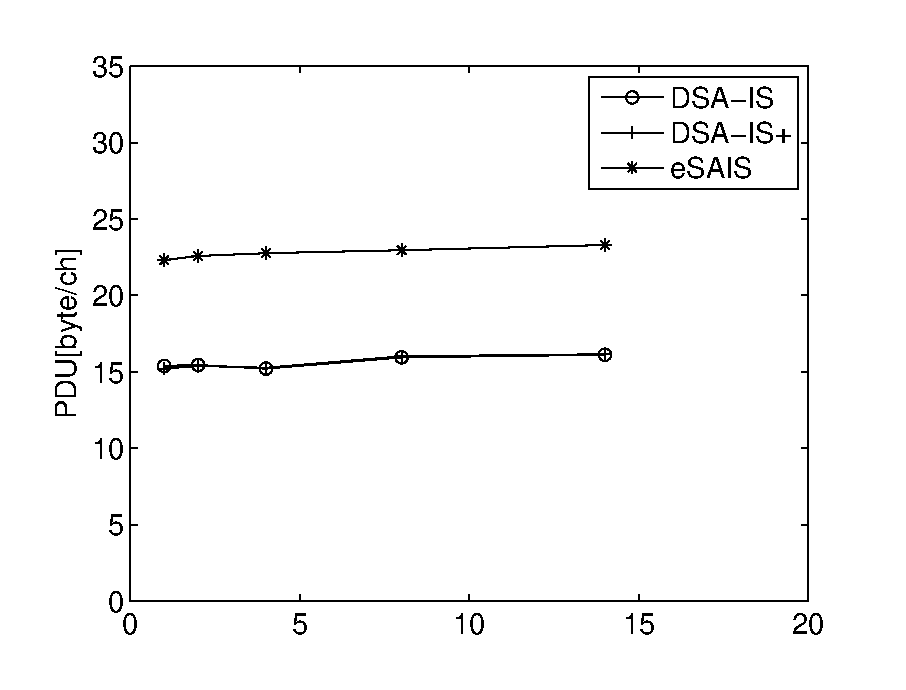
\includegraphics[width=1\textwidth]{pdu_cmp2_guten} \\
			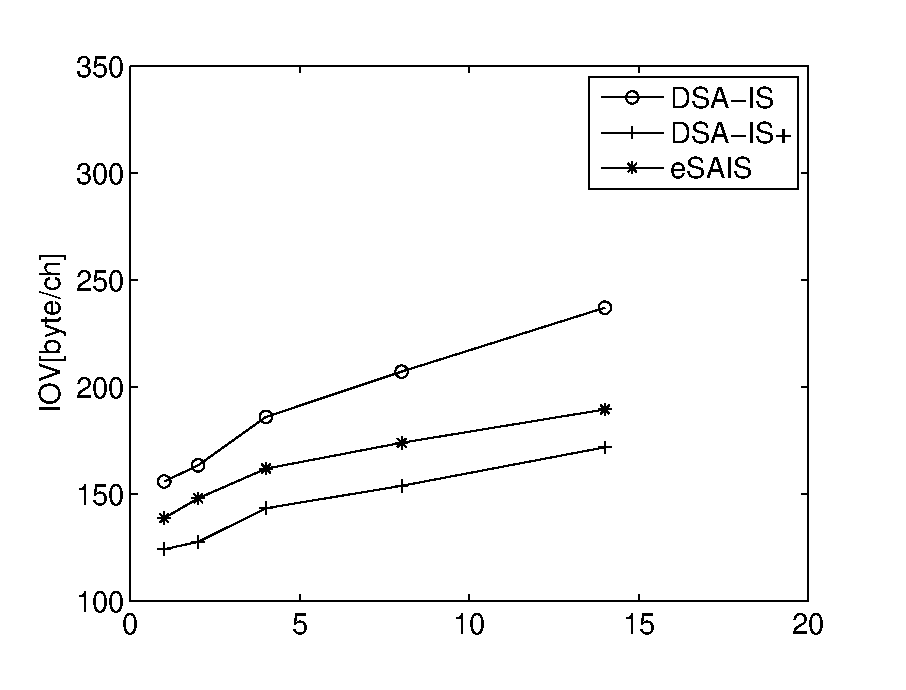
\includegraphics[width=1\textwidth]{iov_cmp2_guten} \\
			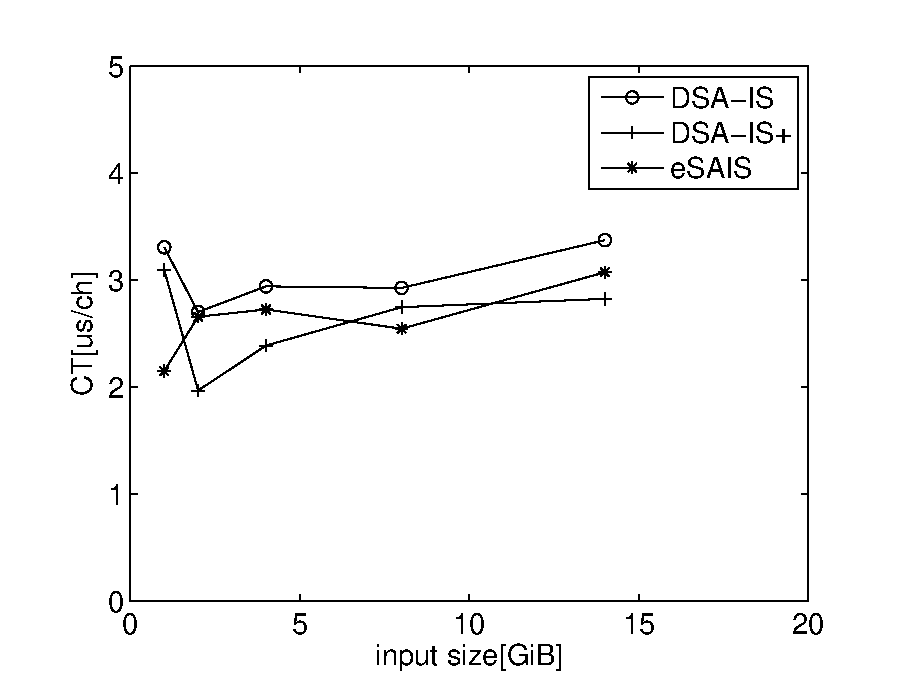
\includegraphics[width=1\textwidth]{ct_cmp2_guten}
		\end{minipage}
	}
	\subfigure[enwiki]{
		\begin{minipage}[b]{0.45\textwidth}
			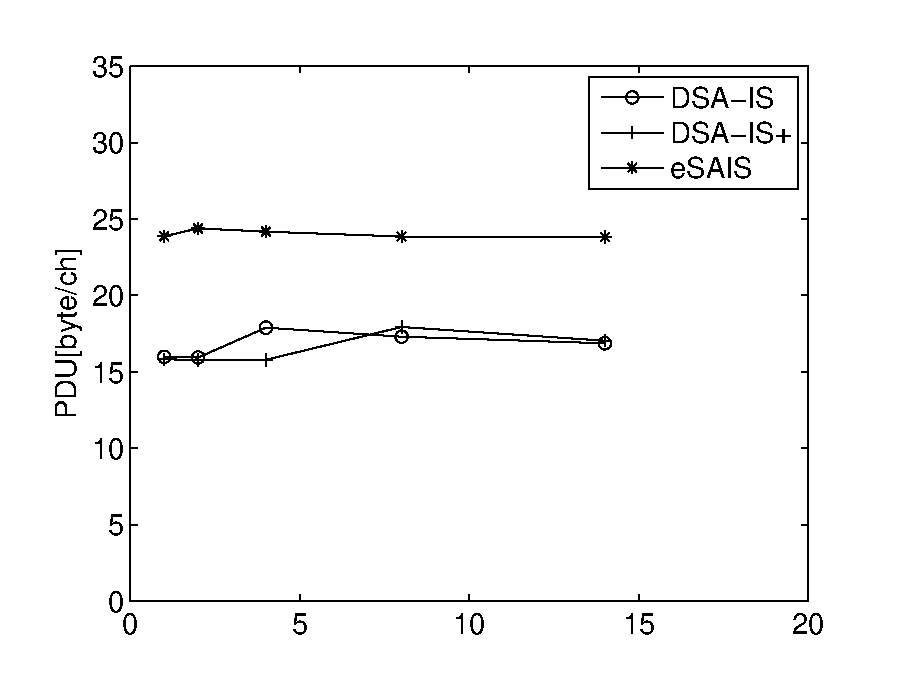
\includegraphics[width=1\textwidth]{pdu_cmp2_enwiki} \\
			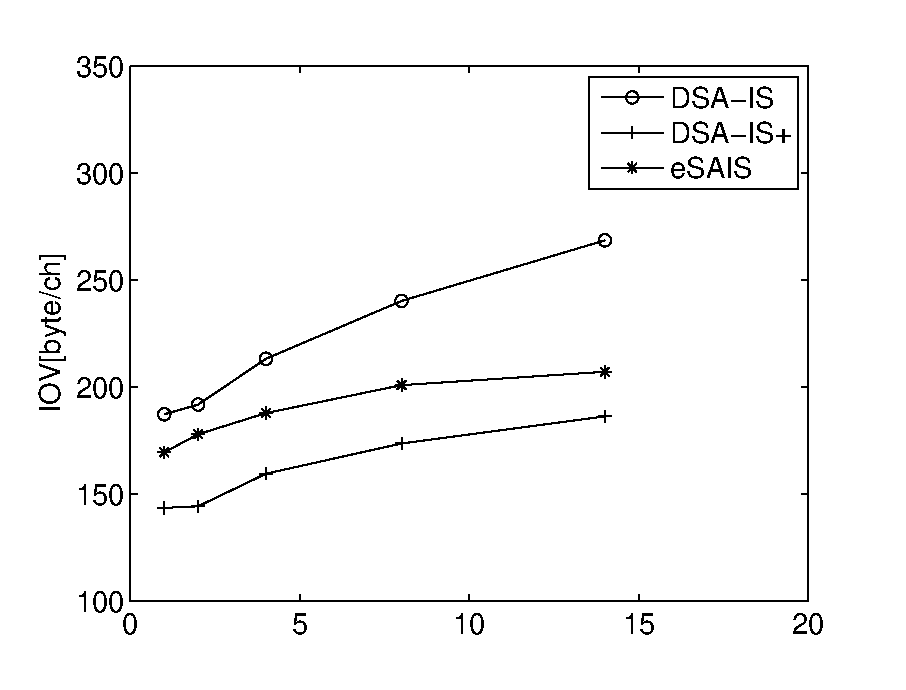
\includegraphics[width=1\textwidth]{iov_cmp2_enwiki} \\
			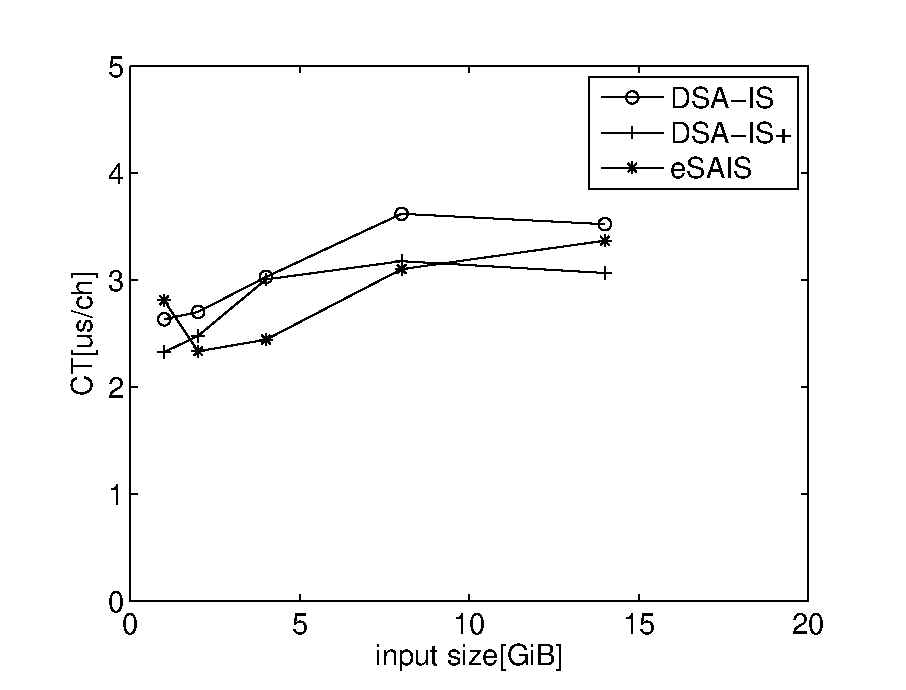
\includegraphics[width=1\textwidth]{ct_cmp2_enwiki}
		\end{minipage}
	}
	\caption{Experimental results for DSA-IS, DSA-IS+ and eSAIS on guten and enwiki in terms of peak disk usage, I/O volume and construction time, where $D_1 = 8$, $D_2 = 10$ and the input size varies in \{1, 2, 4, 8, 14\} GiB. }
	\label{fig:performance_analysis2}
\end{figure*}

%As with other external memory suffix sorting algorithms, DSA-IS+ is I/O-intensive and its construction speed is presumed to be linearly proportional to the I/O volume. However, our experiments indicate that the ratio of the reduction and induction time is much higher than that of the reduction and induction volume. This phenomenon is possibly due to the performance of the STXXL library. For implementation simplicity, we organize the item of DSAITEM arrays by using the sorter and priority queue containers provided by STXXL in our programs. This

A series of experiments are conducted to investigate the effect of $D_1$ and $D_2$ on the performance of DSA-IS+. As shown in Figure~\ref{fig:performance_analysis3}, the time consumption of DSA-IS+ gets smaller as $D_2$ becomes larger, while the peak disk usage and I/O volume are almost unchanged. Furthermore, the data of Table~\ref{tbl:effect_of_D} indicates that a small variation on the values of $D_1$ and $D_2$ can incur a significant fluctuation on the speed of DSA-IS+. For instance, when changing $(D_1, D_2)$ from $(8, 10)$ to $(16, 16)$, the construction time for the uniprot dataset decreases from 2.64 to 2.24 microseconds per character. This is because the proportions of long LMS substrings of $x$ and $\{x1, x2,...\}$ decrease when $D_1$ and $D_2$ increase. Recall that, after partitioning $x$ into blocks, DSA-IS+ sorts the long LMS substrings of each block in RAM and merges them by an external memory sorter, which is time-consuming when the number of long LMS substrings is large. In our program, the ratio of long and short LMS substrings can be controlled by adjusting the values of $D_1$ and $D_2$. However, when $D_1$ and $D_2$ get larger, the min heap also takes more time to merge the sorted short and long LMS substrings, as each string comparison takes $\mathcal{O}(D_1)$ and $\mathcal{O}(D_2)$ time in the first and recursion levels, respectively. Fortunately, Table~\ref{tbl:long_short_distribution} shows that the majority of LMS substrings in real datasets are considerably short. In practice, we can set $D_1$ and $D_2$ according to the statistics of the length distribution of LMS substrings, where the statistics can be collected when partitioning $x$ at the beginning of the reduction phase.

\begin{table*}[htbp]
	\caption{Effects of $D_1$ and $D_2$ for DSA-IS+}
	\label{tbl:effect_of_D}
	\centering
	\begin{tabular}{|c|c|c|c|c|c|c|c|c||c|c|c|c|c|}
		\hline
		\multicolumn{1}{|c}{} & \multicolumn{3}{|c}{eSAIS} & \multicolumn{10}{|c|}{DSA-IS+}\\\hline
		\hline
		Corpora & PDU & IOV & CT & $D_1$ & $D_2$ & PDU & IOV & CT  & $D_1$ & $D_2$ & PDU & IOV & CT\\\hline
		uniprot & 22.71 & 162.01 & 2.50 & 8 & 10 & 14.27 & 146.10 & 2.64 & 16 & 16 & 14.27 & 144.90 & 2.24 \\\hline
		proteins & 24.09 & 172.29 & 2.33 & 8 & 10 & 16.12 & 147.92 & 2.28 & 20 & 12 & 16.12 & 147.85 & 2.14 \\\hline
		genome & 22.64 & 157.41 & 2.15 & 8 & 10 & 15.34 & 142.05 & 2.75 & 20 & 12 & 15.34 & 140.89 & 2.25 \\\hline
	\end{tabular}
\end{table*}%

\begin{figure}[htbp]
	\centering
	\subfigure{
		\centering
		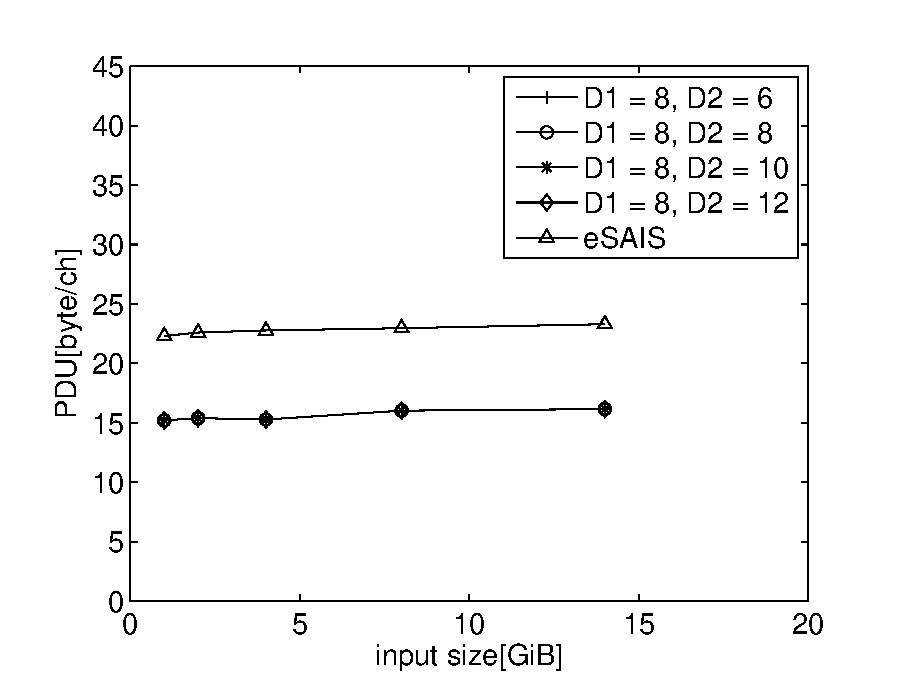
\includegraphics[width=0.9\columnwidth]{pdu_cmp3}
		\label{subfig:pdu_cmp3}
	}
	\hfil
	\subfigure{
		\centering
		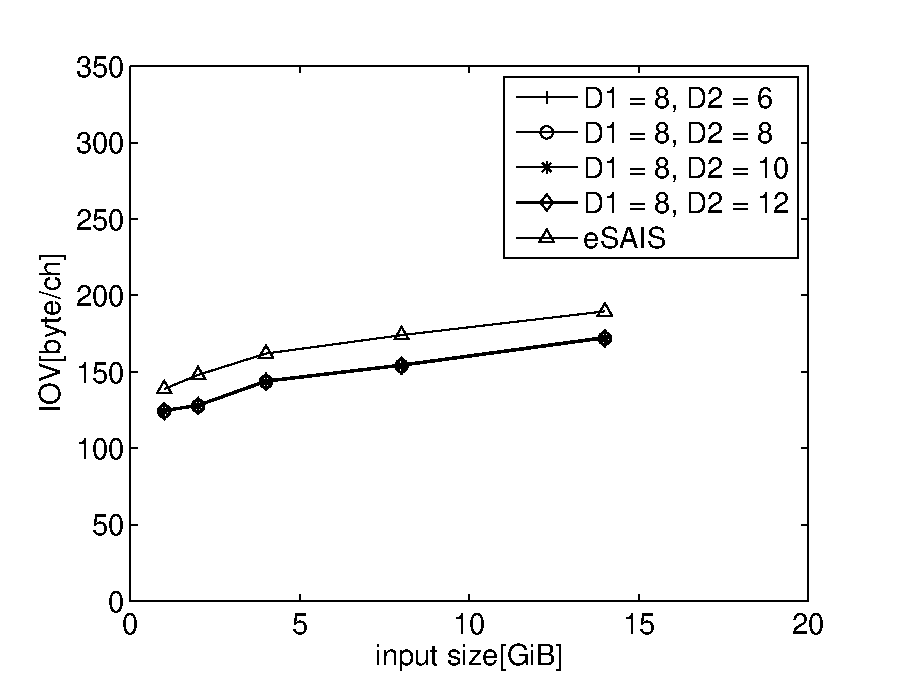
\includegraphics[width=0.9\columnwidth]{iov_cmp3}
		\label{subfig:iov_cmp3}
	}
	\hfil
	\subfigure{
		\centering
		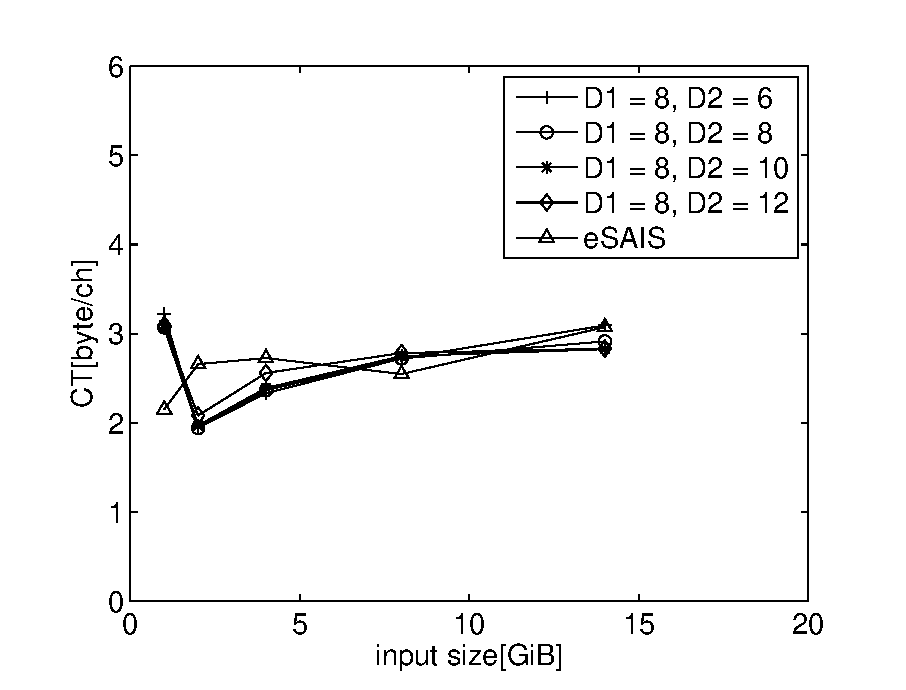
\includegraphics[width=0.9\columnwidth]{ct_cmp3}
		\label{subfig:ct_cmp3}
	}
	\caption{Experimental results for DSA-IS+ and eSAIS on guten in terms of peak disk usage, I/O volume and construction time, where $D_1 = 8$, $D_2$ ranges in \{6, 8, 10, 12\} and the input size varies in \{1, 2, 4, 8, 14\} GiB. }
	\label{fig:performance_analysis3}
\end{figure}


\begin{table*}[htbp]
	\caption{Statistics on the Length Distribution of Long and Short LMS Substrings for DSA-IS+}
	\label{tbl:long_short_distribution}	
	\centering
	\begin{tabular}{|c|c|c|c|c|c|c|c|c|c|c|}
		\hline
		\multicolumn{11}{|c|}{level 0} \\\hline
		Corpora & $D_1$ & long & short & total & ratio & $D_1$ & long & short & total & ratio\\\hline
		uniprot & 8 & 30243605 & 785997413 & 816241018 & 0.963 & 16 & 3850755 & 812390263 & 816241018 & 0.999\\\hline
		proteins & 8 & 1687673 & 377404329 & 379092002 & 0.999 & 20 & 10930 & 379081072 & 379092002 & 0.999\\\hline
		genome & 8 & 19446841 & 773670266 & 793117107 & 0.975 & 20 & 509998 & 792607109 & 793117107 & 0.999\\\hline
		\multicolumn{11}{|c|}{level 1}\\\hline
		Corpora & $D_2$ & long & short & total & ratio & $D_2$ & long & short & total & ratio\\\hline
		uniprot & 10 & 11849 & 263748775 & 263760624 & 0.995 & 16 & 380 & 263760244 & 263760624 & 0.999\\\hline
		proteins & 10 & 18126 & 123772731 & 123790857 & 0.996 & 20 & 2937 & 123787920 & 123790857 & 0.999\\\hline
		genome & 10 & 311607 & 248243216 & 248554823 & 0.999 & 20 & 153845 & 248400978 & 248554823 & 0.999\\\hline
	\end{tabular}
\end{table*}%


\subsection{Performance Evaluation on Checking Methods}

\begin{table*}[htbp]
	\caption{Overall Performance of DSA-IS+ and eSAIS with CM1 and CM2 on enwiki\_8G}
	\label{tbl:check_overhead}
	\centering
	\begin{tabular}{|c|c|c|c|c|c|c|}
		\hline
		& \multicolumn{3}{|c|}{DSA-IS+ ($D_1 = 8$, $D_2 = 10$)} & \multicolumn{3}{c|}{eSAIS}\\\hline
		Checking Method & PDU & IOV & CT & PDU & IOV & CT \\\hline
		CM1 & 17.93  & 180.01 & 3.10 & - & - & - \\\hline
		CM2 & 26.00 & 231.68 & 4.00 & 27.00 & 246.93 & 3.74 \\\hline
		no check & 17.93  & 173.67	& 3.17 & 23.85 & 200.93 & 3.10 \\\hline
	\end{tabular}
\end{table*}%


We make a performance comparison of the proposed checking method and the work presented in~\cite{Karkkainen2003}, which are denoted by CM1 and CM2, respectively. For performance evaluation, we integrate CM1 into the program of DSA-IS+ following Section~\ref{subsec:sachecker:implementation} and reuse the implementation for CM2 in the program of eSAIS to verify the outputs of DSA-IS+ and eSAIS. Table~\ref{tbl:check_overhead} gives a glimpse of the performance overhead for the two checking methods. It can be seen that, when checking the suffix array of enwiki\_8G by using CM2, both time and I/O volume for verification are about one-fifth of that for construction. On the other hand, CM1 has almost no negative impact on the overall performance. As demonstrated in lines 3 and 5, the peak disk usage for CM1 is no more than that for DSA-IS+ and the increase in the I/O volume can be ignored. It worth mentioning that the data of the running time for the combination of DSA-IS+ and CM1 is a bit shorter than that for the plain DSA-IS+. This is a normal phenomenon due to the fluctuating I/O performance, which in turn indicates that the time overhead consumed by CM1 is also negligible.




\section{Conclusion} \label{sec:conclusion}

For better performance, we redesign the reduction phase of DSA-IS by employing two methods for sorting and naming substrings. The program of the enhanced algorithm DSA-IS+ is engineered by the STXXL library to achieve a high I/O efficiency. Our experiments indicate that DSA-IS+ requires only around $16/24=0.67$ peak disk usage as that for eSAIS and runs as fast as the latter on various real datasets.

We describe an SA checker of linear time and space complexities that can be used to verify a suffix array during the time when it is being built. In combination with DSA-IS+, our checking method almost has no influence on the overall performance and is more efficient than the existing work in terms of time, space and I/O efficiencies.

\bibliographystyle{IEEEtran}
\bibliography{IEEEabrv,bibfile}

\end{document}


